

%吉野君
\usepackage{here}

\title{ビッグデータ処理技術を用いたWikipediaマイニング}
\author{プロジェクトマネジメントコース\\
ソフトウェア開発管理グループ\\
矢吹研究室\\
1242005\\
石井康之}
\date{}
\begin{document}
\maketitle

\chapter*{謝辞}

本研究を進めるにあたり,矢吹研究室矢吹太朗准教授には,多くの時間をご指導にさいて頂きました.
また矢吹研究室の皆様には,多くの知識や示唆を頂きました.協力していただい皆様に感謝の気持ちと御礼を申し上げます.

\tableofcontents%目次

\chapter{序論}

当研究はビッグデータ処理技術を用いたWikipediaマイニングを行う.

Wikipediaとは,非営利のWikimedia財団がインターネット上で運営する,無料のオンライン百科事典プロジェクトである.記事の内容はボランティアの人々の協力によって,信頼のおける品質が保たれている.

ビッグデータとは,市販されているツールや従来のデータ処理で行うことが困難なほど巨大なデータ集合の集積物のことである.

先行研究では,{Google BigQuery}という,{Google Cloud Platform}が提供するビッグデータ解析サービスを扱った.{Google BigQuery}のサイトの中に,サンプルデータとして,Wikipediaの編集履歴データを提供していたので、それを用いて研究を行った.しかし,提供されていたデータは英語版だけのものであり,多言語の研究を行うことができなかったので,別の研究方法を検討する必要がある.

そこで当研究は,多言語版Wikipediaもデータ解析できる技術を得るために,ローカルで研究が行える環境を用意し,データマイニングを行う.

Wikipedia の全編集データをマイニングすることによって,Wikipedia の品質が保たれている理由を見つけ出す.



\chapter{背景}

\section{研究背景}
Wikipediaは,多くのボランティアにより,始まってから10年足らずの間に,大きな成長を見せたオンライン百科事典プロジェクトである.総記事数の文字数は10億文字を超え,ブリタニカ国際大百科事典とエンカルタ総合大百科の合計と比較しても上回る.Wikipediaは,さまざまな言語が参加しているグローバルなプロジェクトでもある.2015年9月までには,291個もの言語が参加している.

このオープンなプロジェクトの百科事典は,制限無く誰でも自由に使用でき編集することもできる.

誰でも自由に編集できるからこそ,ボランティアの人々は気軽に参加でき,特定の企業や個人のお金を稼ぐのに力を貸していると感じることなく,時間と労力を注ぐことができる.

記事の内容はボランティアの人々の協力によって,信頼のおける品質が保たれている.しかし,中には協力的では無く,悪意のある編集をするものがいる.悪意のある編集者はその記事の内容とは関係ないことを書き込んだり,記事の破壊行為を繰り返している.Wikipediaでは,悪意のある編集をする人とわかっていても規制などをしたりはしない.記事は完成・確定されることはなく,新しい情報にいつでも改変することができる.

本研究では,Wikipediaの全編集データをマイニングすることによって,Wikipediaの品質が保たれている理由を見つけ出す.



\section{Wikipediaとは}

フリー・ライセンスの百科事典である.フリーには2つの意味がある.無料という意味と,自由という意味だ.Wikipediaのフリーは後者の自由という意味であり,四つの自由が与えられている.著作物を複製する自由.改変する自由.再頒府する自由.そして,改変版を再頒府する自由だ.そして,営利目的に使っても,非営利に使ってもかまわない.というものがある.Wikipediaがフリーの百科事典であるというのは,無料でアクセスできるということではなくて,自由に複製,改変,利用してかまわないということである.

Wikipediaという名前は,ウェブブラウザ上でウェブページを編集することができるWikiというシステムを使用した百科事典であることに由来する造語である.設立者の1人であるラリー・サンガーにより命名された.

Wikipediaは2015年9月までには,291個もの言語が参加している.この百科事典は多くの言語のボランティアたちによって書かれたグローバルなプロジェクトでもある.\cite{wikirevo}



\subsection{記事の編集の仕方}

 一部の保護されているページを除いて,全てのページには「編集」と書かれたリンクがあり,このリンクを使って,あなたが閲覧しているページを編集することができます.編集ができることはウィキペディアの大きな特徴で,この機能を使って,あなたが記事を修正したり,記事に加筆することができるのです.記事に情報を加筆する時には,情報の出典を明記してください.出典が不明な記述は,除去の対象となります.\cite{wikiEdit}

%図の挿入
\begin{figure}[H]
\centering
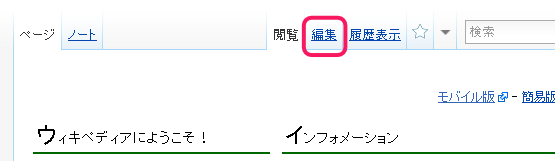
\includegraphics[width=10cm]{sample1.png}
\caption{図の挿入例}\label{サンプル図}
\end{figure}

これから常に使ってほしい大切な機能が「プレビューを表示」ボタンです.サンドボックスでなにか編集をして,それから「以上の記述を完全に理解し同意した上で投稿する」ボタンではなく,「プレビューを表示」ボタンを押してみましょう.そうすると,あなたがページに加えた変更の結果を,実際に保存する前に確認することができます.間違いは誰にでもあります.この機能は,間違いがないか自分で確認するためのものです.また,「プレビューを表示」ボタンを使えば,試しにページの体裁や表現をいろいろと変えてみても,ページの変更の記録にいちいち記録されずにすみますし,他にもいろいろと利点があるのです.でも,プレビューをした後,最後には保存するのを忘れないでください.\cite{wikiEdit}

%図の挿入
\begin{figure}[htb]
\centering
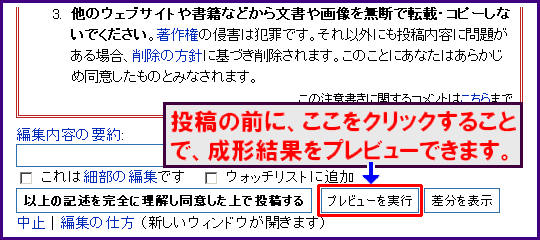
\includegraphics[width=10cm]{sample2.png}
\caption{図の挿入例}\label{サンプル図}
\end{figure}

「以上の記述を完全に理解し同意した上で投稿する」ボタンを押す前に、あなたが行った編集の説明を、編集用のテキストボックスと保存ボタンの間にある要約欄に書き込むようにしましょう。ウィキペディアでは、ここに編集の説明を書き込むことが大切なエチケットと考えられています。ただ単に誤字を直したような時には「誤字修正」と書けば充分です。文章の意味に影響を及ぼさないような、小さな修正のときには、要約欄の下にある「これは細部の編集です(説明)」のチェックボックスにチェックをいれておいてください(この機能はログイン時にのみ有効です)。\cite{wikiEdit}

%図の挿入
\begin{figure}[htb]
\centering

\includegraphics[width=10cm]{sample3.png}
\caption{図の挿入例}\label{サンプル図}
\end{figure}

\subsection{Wikipediaの編集履歴データ}

データCreative Commons Attribution-ShareAlike 3.0 Unported License (CC-BY-SA) および GNU Free Documentation License (GFDL) の下にライセンスされており (Wikipedia:著作権および利用規約を参照),再配布や再利用のためにデータベース・データの提供が行われています.データの生成は不定期に行われている.

Wikipediaではクロール行為のデータダウンロードは禁止されている.強引なクローリングは,Wikipediaが劇的に遅くなる原因となってしますためである.データベースから自動的にデータ収集している行為が発券された場合、システムの管理者から自身のサイトからWikipediaのアクセスを禁止されてしまう措置が起こってしまうこともある.また,ウィキペディア財団が法的措置を検討する場合もあるので,注意が必要.

%図の挿入
\begin{figure}[htb]
\centering
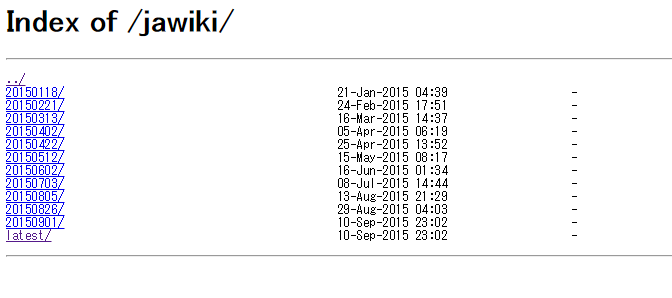
\includegraphics[width=10cm]{sample4.png}
\caption{図の挿入例}\label{サンプル図}
\end{figure}

ここに日本語版Wikipediaの履歴データが記録されている.

URLはhttps://dumps.wikimedia.org/jawiki/

他の言語もこのような形式で履歴データが残されている.他の言語のデータを取得したい場合はURLのhttps://dumps.wikimedia.org/○○wiki/の○○の部分を変更すればよい.言語は英語のスペルで頭文字2文字でよい.

例:英語の場合はスペルはEnglishなので,https://dumps.wikimedia.org/enwiki/とすればよい.



%図の挿入
\begin{figure}[htb]
\centering
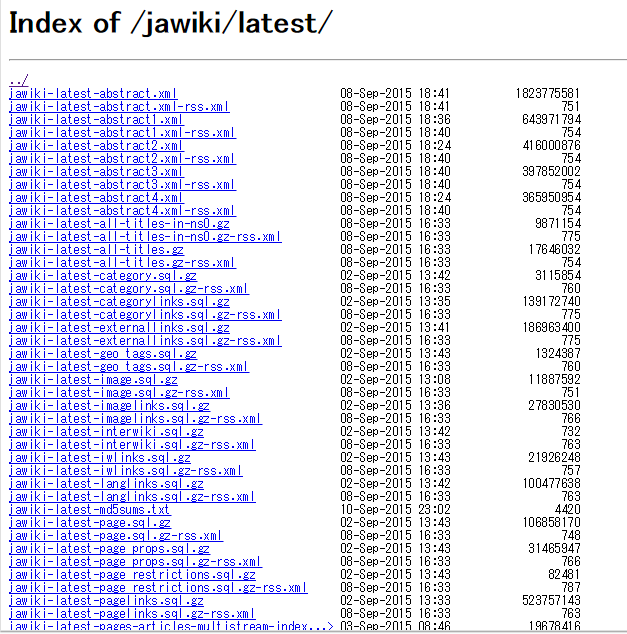
\includegraphics[width=10cm]{sample5.png}
\caption{図の挿入例}\label{サンプル図}
\end{figure}

どれか開くと上記のような画面になる.

ウィキページのデータはSQLのテーブルではなく、XMLで提供されている。XMLファイルの文字エンコーディングはUTF-8である。 非常にファイルサイズが大きいため、通常のエディタやブラウザで、解凍してはいけない。

データの詳細は下記のとおり

\begin{itemize}
 \item pages-articles.xml.bz2 - ノートページ、利用者ページを除く最新版のダンプ
 \item pages-meta-current.xml.bz2 - 全ページの最新版のダンプ
 \item pages-meta-history.xml.7z - 全ページの全ての版のダンプ
 \item all-titles-in-ns0.gz - 全項目のページ名一覧 (標準名前空間)
\end{itemize}

\subsection{Wikipedia:編集回数の多いページの一覧}

期間: 2014-07-01 — 2014-07-31 のランキング.


%図の挿入
\begin{figure}[H]
\centering
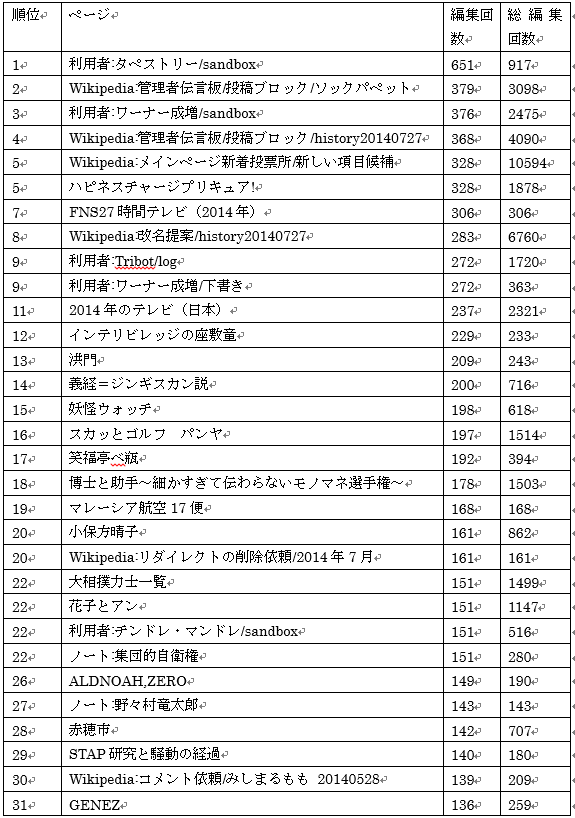
\includegraphics[width=12cm]{sample6.png}

\end{figure}


%図の挿入
\begin{figure}[H]
\centering
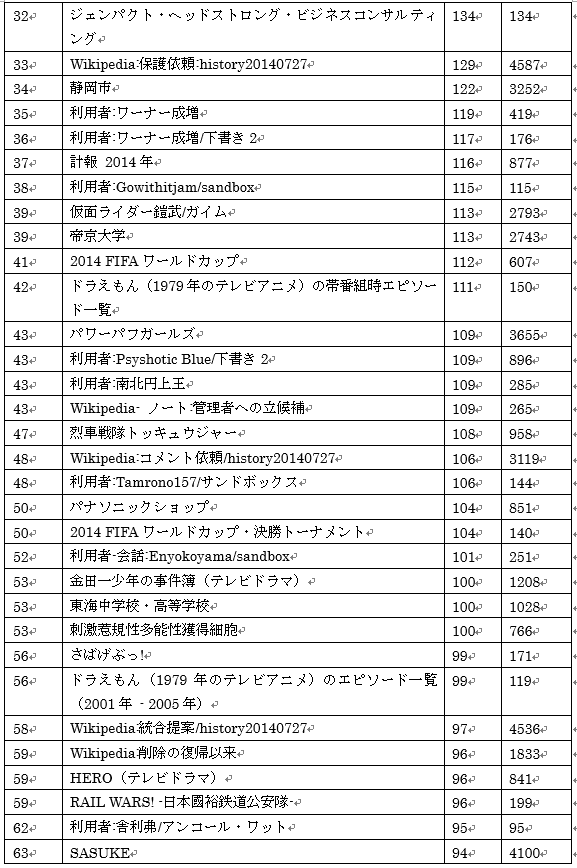
\includegraphics[width=12cm]{sample7.png}

\end{figure}


%図の挿入
\begin{figure}[H]
\centering
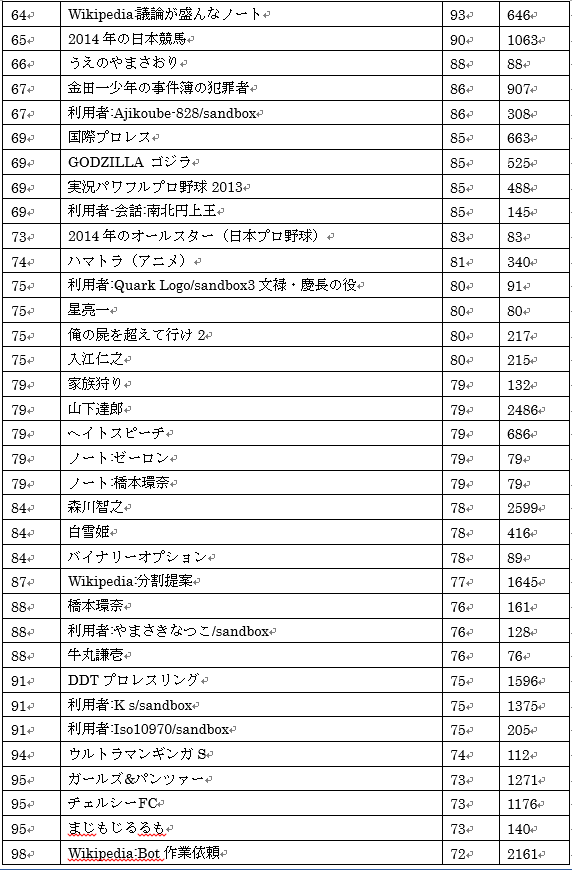
\includegraphics[width=12cm]{sample8.png}

\end{figure}


%図の挿入
\begin{figure}[H]
\centering
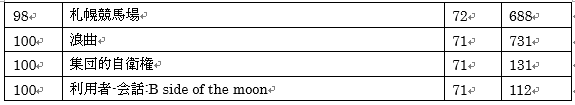
\includegraphics[width=12cm]{sample9.png}

\end{figure}

ビッグデータとは

パソコン,スマートフォンが普及し「ビッグデータ」という言葉が流行することからもわかるように,私たちは膨大な情報を日々生み出しながら生活している.GoogleやYahoo!に寄せられる大量の検索クエリや,Twitter,FacebookなどのSNSに投稿される文章や画像,動画,スマートフォンを利用するサービスなどで収集される位置情報データ,防犯カメラで記録される人間の表情や動きのデータなどの膨大な量のデータを指す.

ビッグデータとは,一般的にペタ(1,000兆),バイト級のデータ量といわれている.このような数値的定義もあるが,ペタバイト以下であればビッグデータではないという訳でもなく,本質的には,「従来の手段では管理しきれない規模のデータ」を指す.

\begin{table}[H]
  \begin{tabular}{|c|c|c|c|l|c|} \hline
    $10^n$ & 接頭辞 & 記号 & 漢数字表記 & 十進数表記 & 分類 \\ \hline
    $10^21$ & ゼタ(zetta) & Z & 十垓 & 1,000,000,000,000,000,000,000 & ビッグデータ \\ \hline
    $10^18$ & エクサ(exa) & E & 百京 & 1,000,000,000,000,000,000 & ビッグデータ \\ \hline
    $10^15$ & ペタ(peta) & P & 千兆 & 1,000,000,000,000,000 & ビッグデータ \\ \hline
    $10^12$ & テラ(tera) & T & 一兆 & 1,000,000,000,000 &  \\ \hline
    $10^9$ & ギガ(giga) & G & 十億 & 1,000,000,000 &  \\ \hline
    $10^6$ & メガ(mega) & M & 百万 & 1,000,000 &  \\ \hline
    $10^3$ & キロ(kilo) & K & 千 & 1,000 &  \\ \hline
  \end{tabular}
\end{table}




4VによるBigDataの定義

IBMによるBigDataの定義で4Vというものがある.4Vとは,容量(Volume),種類(Variety),頻度・スピード(Velocity),正確さ(Veracity)から構成されている.



容量(Volume)

ビッグデータの特徴である容量の巨大さを指す.企業内外にはデータが溢れており,数テラバイトから数ペタバイトにもおよぶ.またデータが増大することによる計算量も非常に膨大となる.



種類(Variety)

ビッグデータは企業システムで通常扱っているような顧客情報や販売データ,経理データ,在庫データなどの構造化データであるとは限らない.テキスト,音声,ビデオ,ページ遷移,ログファイルなどのさまざまな種類の非構造化データも存在する.



頻度・スピード(Velocity)

今この瞬間にも,ものすごい頻度でRFIDなどのICタグやセンサーなどからデータが生成されている.昨今の変化の著しい市場環境では,これらのデータによりリアルタイムに対応したものを求められている.



正確さ(Veracity)

データの矛盾,曖昧さによる不確実性,近似値を積み重ねた不正確さなどを排除して,本当に信頼できるデータが意思決定には重要である.



以上がIBMによる4Vの定義であるが,容量(Volume)については最初に記述したように,必ずしもペタバイト以上でなければならないとは考えていない.


%図の挿入
\begin{figure}[H]
\centering
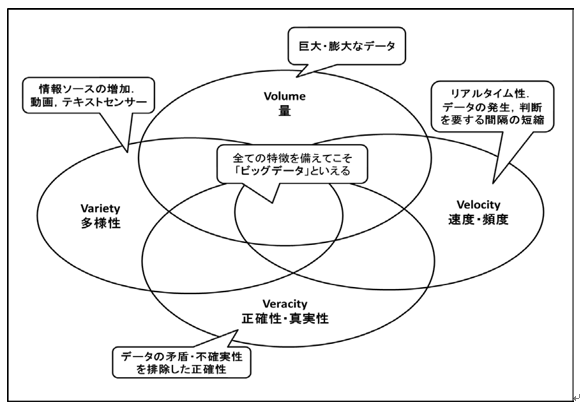
\includegraphics[width=10cm]{bigdata4v.png}
\caption{ビッグデータの4V}\label{サンプル図}
\end{figure}



3Vでのビッグデータの定義

3Vで表す場合は,容量(Volume),種類(Variety),頻度・スピード(Velocity)の3つになり,正確さ(Veracity)は含まれない.確かにビッグデータには正確でないデータが混在することもあり,例えばTwitterなどのSNSデータには,冗談やデマ情報の書き込みなども混じっており,センサーなどでも故障によるノイズが混じることもあります.データ量が少ない場合には,外れ値として手作業で除去することも可能だがいわゆるビッグデータと言われている大量のデータの場合は,手作業によるデマ情報やノイズなどの除去はほとんどふかのうである.

しかし,ビッグデータで収集するデータは殆どが生データであるという特徴がある.正確さをどう定義するにもよるが,センサーからの入力データなどは生データそのものだが,SNSからの入力データなども生データであり,その意味では正確なデータといえる.つまり,編集などで手が加わっていないデータであり,またそこで発せられるメッセージはその人が,その人の環境により制約などを感じるデータではないからだ.これは,勤務する企業・組織内で作成する報告書などと対比して考えるとわかりやすいだろう.


ビッグデータ処理のパターン

下記の表に,3つの処理パターンの特性を簡潔にまとめたものを記述する.

\begin{table}[H]
  \begin{tabular}{|l|l|l|l|} \hline
                     & バッチ処理 & インタラクティブクエリー処理 & ストリームデータ処理 \\ \hline
    実行タイミング & ユーザー指定と定期的実行 & ユーザー指定と定期的実行 & 常時連続実行 \\ \hline
    処理単位 & 蓄積データをバッチで一括処理 & 蓄積データをバッチで一括処理 & 少数のフローデータ処理 \\ \hline
    実行時間 & 分~時間 & 秒~分 & ミリ秒~秒 \\ \hline
    処理モデル & MapReduce & クエリ・OLTP & ストリーム処理 \\ \hline
  \end{tabular}
\end{table}


ビッグデータの処理パターンには,「バッチ処理」,「インタラティブクエリー処理」,「ストリームデータ処理」の3種類のパターンがある.

 バッチ処理では筑西データをバッチで一括処理だが,これはGoogle検索用に開発されたMapReduce処理を利用したHadoopが代表的である.しかし,Hadoopはビッグデータ処理用として開発されたものではないので,処理結果作成に時間がかかるという欠点がある.

インタラティブクエリー処理は,蓄積された大容量データをオンラインクエリなど使用して一括解析処理するものである.インタラティブクエリー処理では蓄積されたビッグデータを数秒から数分で実行する.

ストリームデータ処理は大量発生する実世界データを逐次に時系列処理する技術である.データ発生時にあらかじめ登録したシナリオにしたがって集計・分析に必要なデータを抽出し,データ処理を行う.このように逐次時系列でデータ処理できることから,最新の情報,その中での特異な値の発生などに対してリアルタイムに対応するシステムを構築できることが特徴でIoTへの応用に最適な処理方法といえる.\cite{bigquerystart}


バッチ処理

最初にMapReduceで代表される,バッチ処理の特性を見る.

数十年前のメインフレームは,主記憶が数百キロバイト,価格は数千万程度だった.これを現在のPC(主記憶数ギガバイト,価格は10万円程度)と比べた場合,価格性能比では約100万倍にもなる.また,CPU処理スピードと,ネットワークの帯域幅についてはそれぞれ,主記憶と類似の性能向上を遂げてきている.

このようなことは,コンピューター関係以外の業種ではまったく例を見ない群を抜く性能向上である.この急激なプラットホームの真価がクラウドコンピューティングやそのうえで実行されるビッグデータ処理などを可能にしている.\cite{bigquerystart}

ただし,これはクラウドなどに限ったことではない.ITの世界ではこれまでも短いタイムスパンで新しいテクノロジー・ブレークスルーやビジネスモデルが出現してきており,これはプラットホームやネットワークの新派に依存している部分が多くある.言葉を変えれば,これらの新しい発想はその時点でのプラットホーム性能で初めて成り立つものであり,これをわずかでも前の世代に思いついたとしても,実現不可能である場合が多い.

このようにクラウドなどの先端ITシステムは,現在のそしてこれからも進化を続けるはずのプラットホームやネットワークに依存したものである.\cite{bigquerystart}


インタラティブクエリー処理

インタラティブクエリー処理は,BigQueryによる説明を記述する.Googleがリリースするソフトウェアツールには,もともとGoogleが社内使用の目的で開発していたものも多く,BigQueryもそれに当てはまる.Googleも当初は社内使用でもMapReduceを使用してビッグデータ処理を行っていたが,バッチ処理による結果生成の遅延や処理を行うための準備の煩雑さなどから,それに代わるツールとして開発されたのがBigQueryである.
BigQueryはデータの入力はまたはJSONフォーマットのファイルから直接行うことができる.また,Cloud Storageからのデータロードも可能である.ビッグデータの解析や絞込みはRDB(Relational Database)のSQLに類似したクエリ言語を使用し,UI画面やPCのコマンドラインから容易にデータ検索を行うことができる.他にもExcelを使用し検索・表示を行うことが出来る.\cite{bigquerystart}


%図の挿入
\begin{figure}[H]
\centering
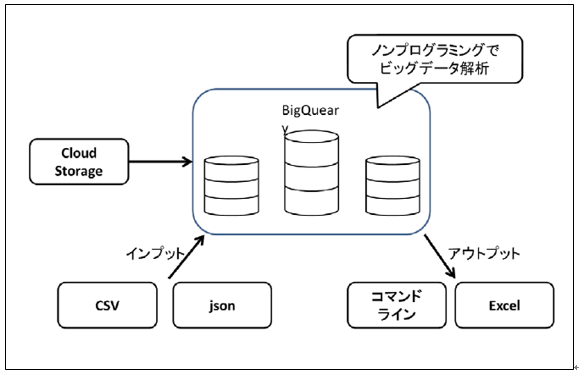
\includegraphics[width=10cm]{bigqueryinout.png}
\caption{BigQueryの入出力}\label{サンプル図}
\end{figure}


BigQueryを使用したインタラクティブクエリ処理では,マウス操作と簡単なキー入力によって全ての操作を行うことができる.また結果出力も数秒から数分以内で得ることができる.したがって,何かこのデータを解析したいと考えたとき,その場で気軽に行えるという点が一番の特徴として挙げられる.

BigQueryでのビッグデータ解析は大量のデータを超高速で行えるのも大きな特徴である.例として,15億行のデータに対する比較的複雑な集計問い合わせが20秒から25秒で返ってきたというユーザの実行結果もある.BigQueryでは,インデスクを作成する必要がなくデータをロードするだけでこのような高速クエリが実行できる.キャッシュは戸鶴ボタンから有効無効を切り替えられるが,キャッシュを使っていなくても,使っているばあ地と同様の結果が得られる.\cite{bigquerystart}



ストリームデータ処理

ストリームデータ処理は,大量発生する時系列のデータ(ストリームデータ)をリアルタイムに逐次処理する技術.

ストリームでたー処理は,データ発生時に,あらかじめ登録したシナリオにしたがって集計・分析に必要なデータを抽出し,データ処理を行う.その際,分析対象データをメモリー上で処理する「インメモリデータ処理技術」により,高速なデータ処理を実現している.これらの技術によって,大量データを高速に,かつリアルタイムに処理できる.例えば,株価のテクニカル指標やランキング情報から売買をリアルタイムに自動判定する.といったシステムに大変有効である.他にも,リアルタイムの在庫管理や,不正操作の監視を行うシステムなど,多くの利用目的が考えられる.\cite{bigquerystart}

%図の挿入
\begin{figure}[H]
\centering
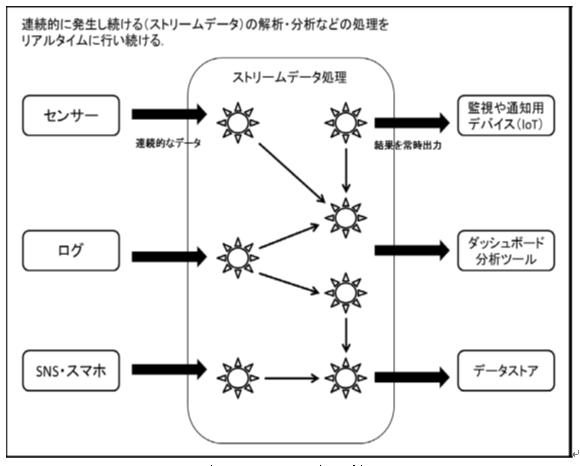
\includegraphics[width=10cm]{streamdatasyori.png}
\caption{ストリームデータ処理}\label{サンプル図}
\end{figure}





\chapter{目的}

研究目的

Wikipediaを一つのプロジェクトとみなし,このオンライン百科事典で品質管理がどのように行われているか調査する.この調査により,オープンな共同作業プロジェクトにおける,品質管理マネジメントのあり方についての知見を得たい.


プロジェクトマネジメントとの関連

本研究は,プロジェクトマネジメントを学ぶことを目的としているため,プロジェクトマネジメントとの関連が全面的にある.

考案するゲームは,プロジェクトマネジメント知識体系ガイド(PMBOK@ガイド)の第4版(以下,PMBOK)を参考にし,プロジェクトマネジメントとの一連の活動や,PMBOKに記載されている9つの知識
エリアについての内容を活用する.\cite{PMBOK}

PMBOKとは,プロジェクトマネジメントに関する知識体系である.

現在は,PMBOKに従ってプロジェクトマネジメントを実施することが,デファクトスタンダードになっている.

PMBOKに記載されている9つの知識エリアとは,何をやるべきかという観点,何を管理するべきかという観点からみたものである.

9つの知識エリアは,以下9つのマネジメントについての内容となっている.


\begin{enumerate}
 \item プロジェクト統合マネジメント
 \item プロジェクト・スコープ・マネジメント
 \item プロジェクト・タイム・マネジメント
 \item プロジェクト・コスト・マネジメント
 \item プロジェクト品質マネジメント
 \item プロジェクト人的資源マネジメント
 \item プロジェクト・コミュニケーション・マネジメント
 \item プロジェクト・リスク・マネジメント
 \item プロジェクト調達マネジメント
\end{enumerate}








本研究では,上記のPMBOKの中の品質マネジメントが関連性が最もあるものであるといえる.このオープンなプロジェクトの百科事典は記事の作成や,編集が主に行われて創り上げられており,その成果物がこの百科事典である.


成果物のイメージ
 差し戻しに関するデータを収集し,編集回数や頻度などの要素を洗い出す.そして,いくつかの要素から条件を決めクラスター分析を行う.その結果から悪意のある編集がされている記事に共通する点を見つけ,Wikipediaのオープンなプロジェクトでの品質マネジメントの知見を得る.




\chapter{手法}

研究方法

\begin{enumerate}
 \item Wikipedia日本語版の編集履歴まで含んだファイルをダウンロードし,ローカルでデータマイニングを行う.
 \item どのような品質管理が行われているか,分析結果から調査を行う.
 \item オープンなプロジェクトにおける品質管理マネジメントのあり方を提案する.
\end{enumerate}

研究を行うための用意

開発環境としてLinuxを扱う.そのために,VirtualBoxとCentOSを用意する. 



VirtualBoxとは

使用しているパソコン上に仮想的なパソコンを作成し,別のOSをインストール・実行できるフリーのパソコン仮想化ソフトのことである.本研究では,LinuxOSを扱いたいが,パソコン本体はWindowsOSの為,このソフトを利用する.


%図の挿入
\begin{figure}[H]
\centering
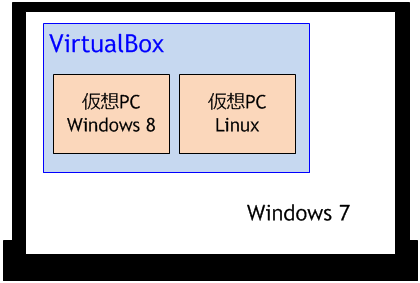
\includegraphics[width=10cm]{sample10.png}
\caption{図の挿入例}\label{サンプル図}
\end{figure}





VirtualBoxはコンピュータ上で直接動作している通常のOSにとってはアプリケーションの一つであり,他のソフトと同じように起動することができる.起動すると仮想的なコンピューターが構築され,元のOSとは独立に別のOSを起動することができる.VirtualBoxが実行されているOSをホストOS,VirtualBox上で実行されているOSをゲストOSという.

元は独立系のソフトウェア企業が開発・販売していた製品だった.しかし,開発元がSun Microsystems社に買収され,その後同社がOracle社に買収されたため,Oracle社が開発元となり,正式名称も「Oracle VM VirtualBox」となった.また,VirtualBox本体はGPLに基づいたオープンソースソフトウェアとして公開され,誰でも自由に入手・利用・改変・再配布などが行える.

VirtualBoxを使う上での注意点

現時点でのVirtualBoxは仮想メモリをサポートしていないため,実メモリ以上のメモリを仮想PCが使用することはできない.仮想メモリを使うと動作が遅くなるため,仮想PCには実メモリ以内のサイズを割り当てる.そのため,仮想PCを1台だけ起動するのであれば問題ないが,複数の仮想PCを同時に起動させる場合これがネックになってしまう.同時起動させる全ての仮想PCのメモリサイズの合計が実メモリのサイズを超えないようにする.そのため,VurtualBoxをインストールするPCには多くのメモリが必要で,最低4GB以上のPCを使うようにするべきである.



\section{VirtualBoxのインストール}

\subsection{ダウンロード}

Oracleが提供しているOracleVitualBoxというのを下記のサイトからダウンロードする.本研究ではWindowsOSを使用しているので,VirtualBox platform packagesの中にある「VirtualBox 5.0.4 for Windows hosts」 というのを選択する.

%図の挿入
\begin{figure}[H]
\centering
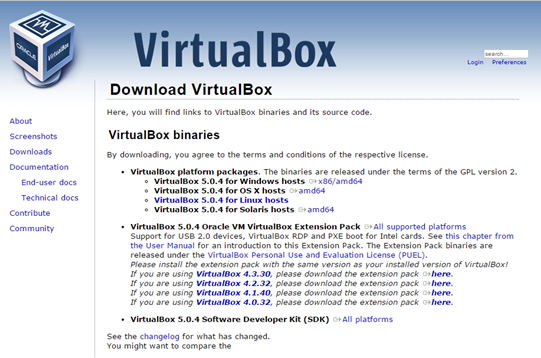
\includegraphics[width=13cm]{VitualBox.png}
\caption{図の挿入例}\label{サンプル図}
\end{figure}


ダウンロードサイト

https://www.virtualbox.org/wiki/Downloads


\subsection{インストーラーの実行}

下記のサイトからVirtualBoxの導入からOSインストールまでの解説が載ってるので参考にする.

%図の挿入
\begin{figure}[H]
\centering
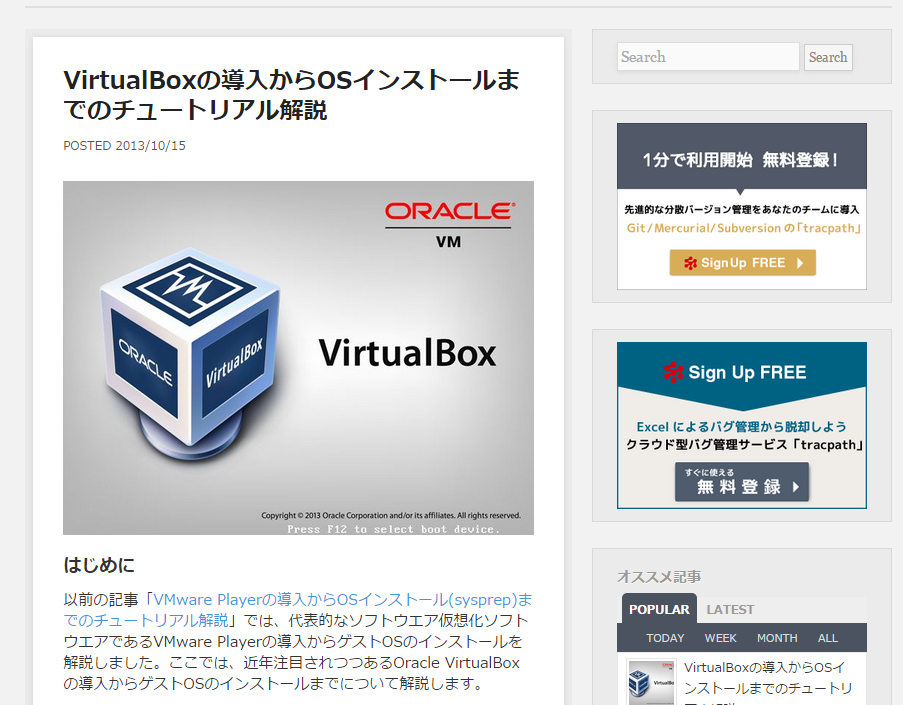
\includegraphics[width=13cm]{sample12.png}
\caption{図の挿入例}\label{サンプル図}
\end{figure}

参考サイト

http://success.tracpath.com/blog/2013/10/15/virtualbox%E3%81%AE%E5%B0%8E%E5%85%A5%E3%81%8B%E3%82%89os%E3%82%A4%E3%83%B3%E3%82%B9%E3%83%88%E3%83%BC%E3%83%AB%E3%81%BE%E3%81%A7%E3%81%AE%E3%83%81%E3%83%A5%E3%83%BC%E3%83%88%E3%83%AA%E3%82%A2/


\section{Ubuntuのインストール}

\subsection{ISOイメージをダウンロードする}

まず,https://www.ubuntulinux.jp/download/ja-remix よりUbuntu 14.04 のISO イメージをダウンロードする.本研究では64bit 版を選択した.



%図の挿入
\begin{figure}[H]
\centering
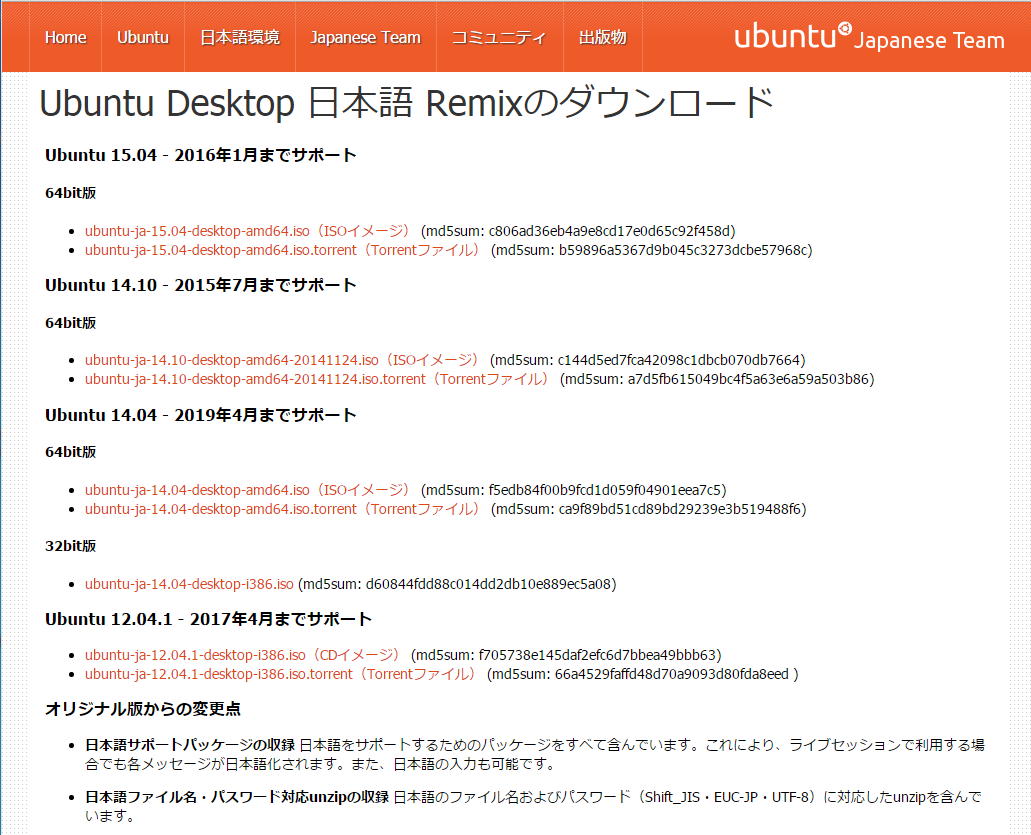
\includegraphics[width=10cm]{UbuntuDL.png}
\caption{UbuntuのISOイメージダウンロードページ}\label{サンプル図}
\end{figure}





\subsection{インストールを開始する}

次にインストールしたVirtualBox を立ち上げ,ウインドウ左上にある「新規(N)」のボタンを押してゲストマシンの作成を行う.ゲストマシンの名前,メモリサイズ,HDD の設定をするとウィンドウが閉じられる.

%図の挿入
\begin{figure}[H]
\centering
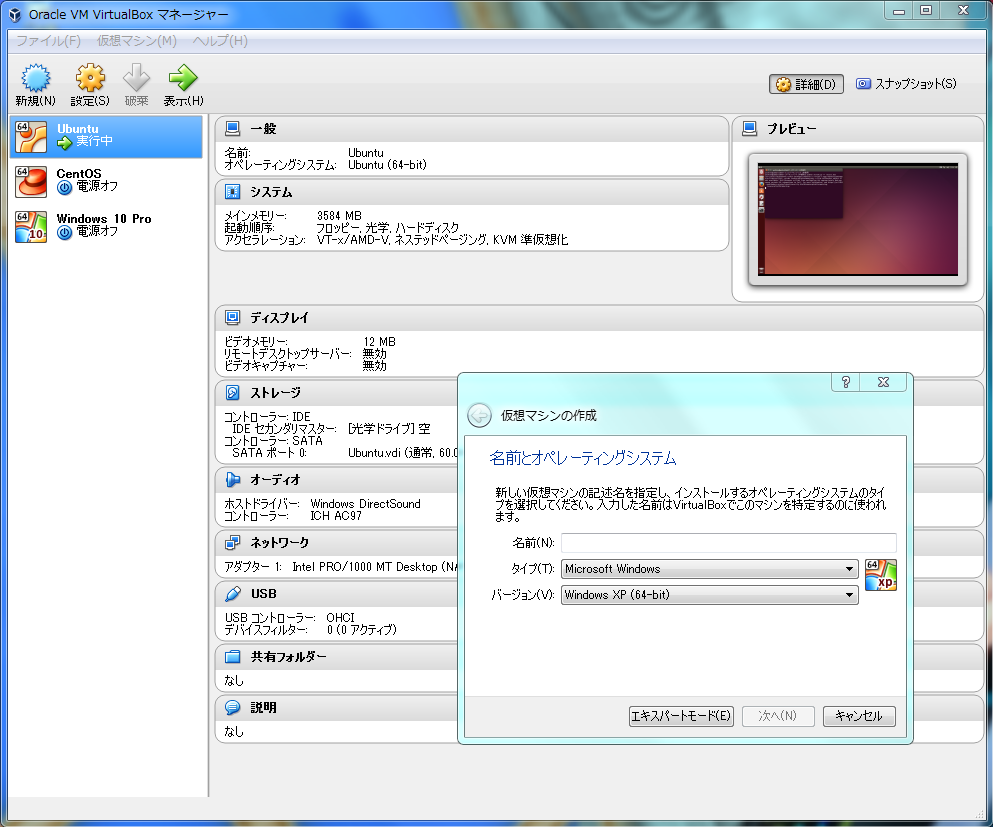
\includegraphics[width=12cm]{VBoxWindow.PNG}
\caption{VirtualBox のウィンドウとゲストマシン作成ウィンドウ}\label{サンプル図}
\end{figure}

続いて「設定(S)」を開き,「ストレージ」の項目からダウンロードしたISO ファイルをセットして「OK」をクリックする.

「起動(T)」を押すとゲストマシンが起動し,Ubuntu のインストールウィザードが表示される.

表示内容に従ってウィザードを進めていくと,ゲストマシン内にUbuntu がインストールされる.


%図の挿入
\begin{figure}[H]
\centering
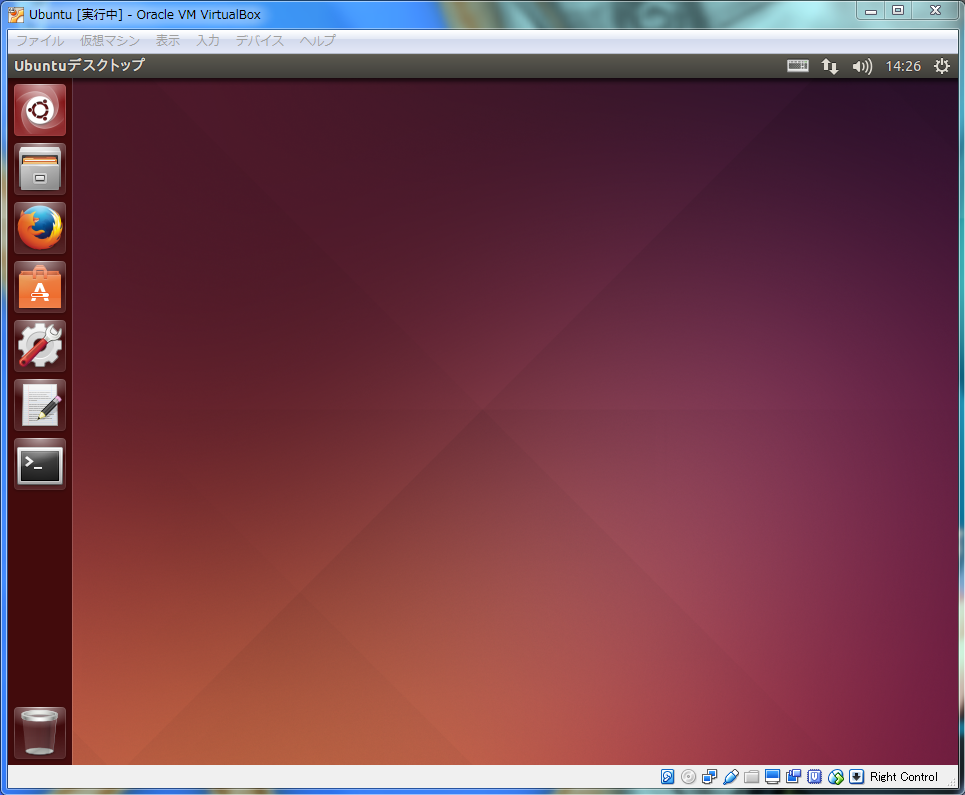
\includegraphics[width=14cm]{Ubuntu_on_VirtualBox.PNG}
\caption{VirtualBox 上で動作するUbuntu}\label{サンプル図}
\end{figure}


\section{Wikipediaの編集履歴データの取得}

\subsection{ファイルのダウンロード}

日本語版Wikipediaのデータは,https://dumps.wikimedia.org/jawiki/からダウンロードできる.

%図の挿入
\begin{figure}[H]
\centering
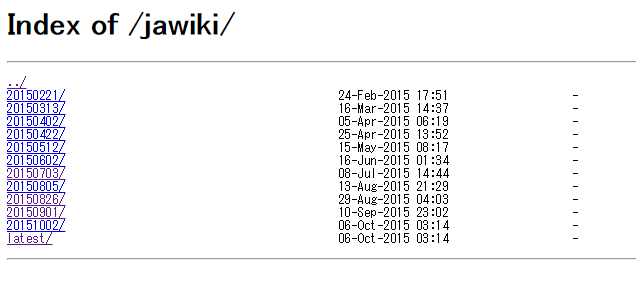
\includegraphics[width=14cm]{Index_of_jawiki.PNG}
\caption{日本語版Wikipediaデータダウンロードサイト}\label{サンプル図}
\end{figure}

再現性を確保するため,20150901番を扱う.latestだと,最新だが,日々更新されて変更されてしまう可能性があるため今回は利用しない.


http://www.mwsoft.jp/programming/munou/wikipedia\_data\_list.htmlによると,stub-meta-history.xmlが使えそうなので,これを利用する.

%図の挿入
\begin{figure}[H]
\centering
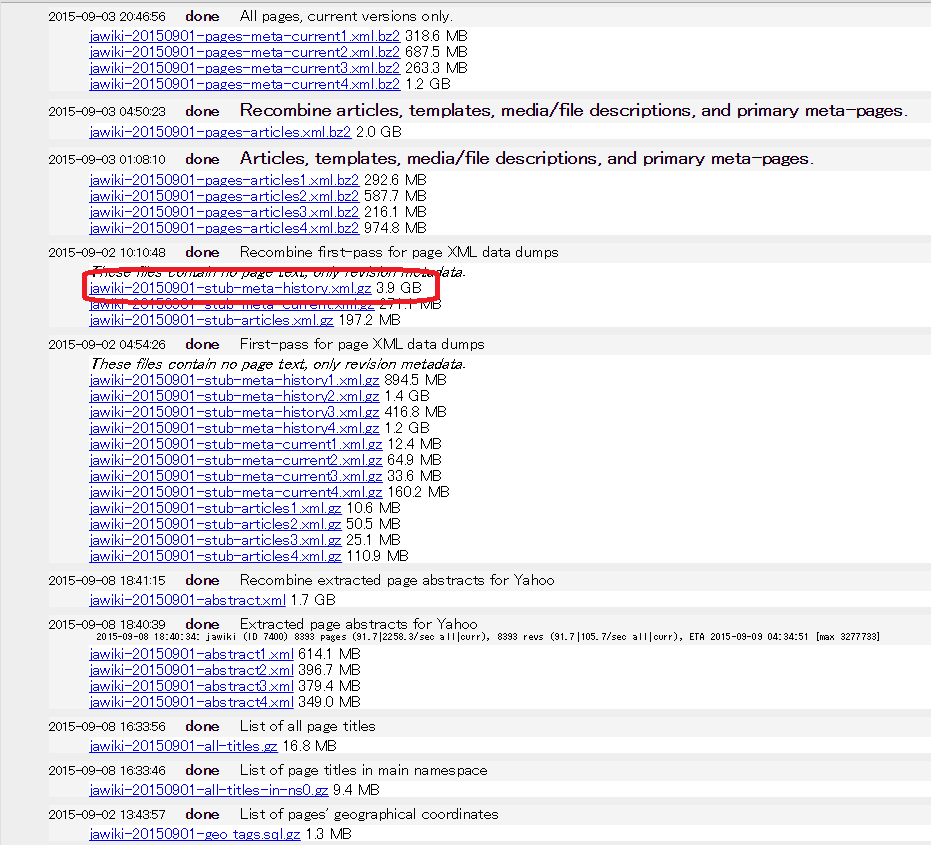
\includegraphics[width=14cm]{wiki20150901.PNG}
\caption{20150901のstub-meta-history}\label{サンプル図}
\end{figure}



\chapter{結果}

\chapter{考察}

\chapter{結論}

%図の挿入
\begin{figure}[htb]
\centering
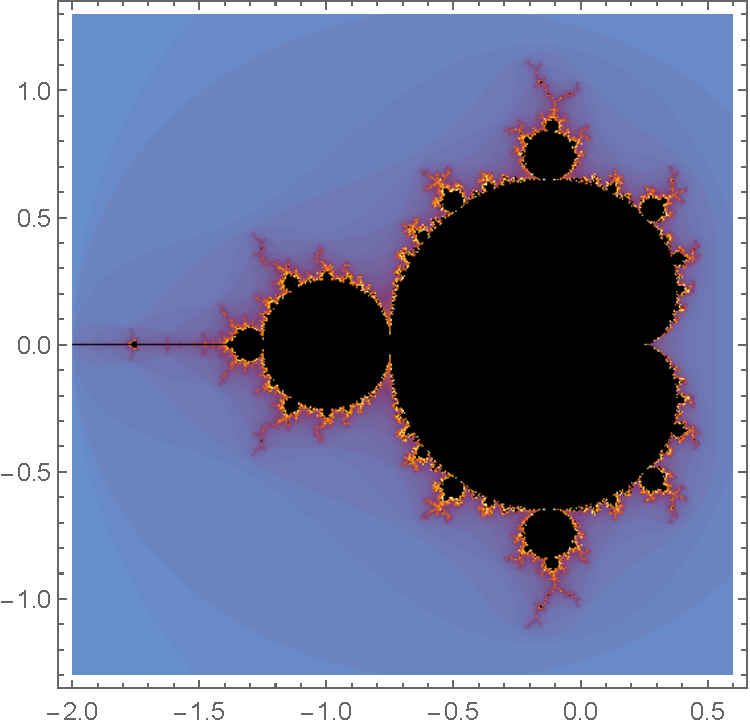
\includegraphics[width=10cm]{figure.pdf}
\caption{図の挿入例}\label{サンプル図}
\end{figure}

参考文献は文献ファイル(この文書では\verb|biblio.bib|)に記述し,\verb|\cite|で参照する.例:データベースのための問い合わせ言語SQLで数独を解く方法が提案されている\cite{yabuki2011}.このように参照すると,参考文献リストに自動的に登録される.文献の種類には,雑誌論文\cite{yabuki2011}や会議録論文\cite{yabuki2013},卒業論文\cite{kubo2014},書籍\cite{okumura2013},ウェブサイト\cite{self}などがある.文献の種類によって必要な項目が異なるため,\verb|biblio.bib|を見て確認すること.

\bibliographystyle{junsrt}
\bibliography{biblio}%「biblio.bib」というファイルが必要.

\end{document}